% ======================= Pre-Amble =========================

\documentclass[11pt, oneside]{article}   	% use "amsart" instead of "article" for AMSLaTeX format 
                     						%imports package {article} and specify option(s) [11pt, oneside]
\usepackage{geometry}                		% See geometry.pdf to learn the layout options. There are lots.                                        

\geometry{letterpaper}                   		% ... or a4paper or a5paper or ... 
%\geometry{landscape}                		% Activate for rotated page geometry

\usepackage[parfill]{parskip}    		        % Activate to begin paragraphs with an empty line rather than an indent

\usepackage[hidelinks]{hyperref}                % Allows for clickable references

%American Mathematics Society packages
\usepackage{amsmath}	   %math
\usepackage{amssymb}       %symbols
\usepackage{amsthm}          %theorems

%Graphics
\usepackage{graphicx}
\usepackage[usenames, dvipsnames]{color}     % font colour:    \textcolor{<colour>}{text}
      									%highlight text:  \colorbox{<color>}{text}
									
									%list of colours: https://www.sharelatex.com/learn/Using_colours_in_LaTeX

%Images		                
\graphicspath{ {images/} }                          %directory that your images are located in within your current directory
	

%Footnote Spacing
\setlength{\footnotesep}{0.4cm}                  %specify spacing b/w footnotes
\setlength{\skip\footins}{0.6cm}                    % space b/w footnotes and textbody

%Table
\usepackage[none]{hyphenat}                    % Stops breaking-up words in a table (i.e. no hyphens)
                                                               

\usepackage{array}   
\newcolumntype{x}[1]{>{\centering\let\newline\\\arraybackslash\hspace{0pt}}p{#1}}       %center fixed column width: x{<len>}                      
\newcolumntype{$}{>{\global\let\currentrowstyle\relax}}                                                   % let us apply things (e.g. bold/italicize) to entire row            
\newcolumntype{^}{>{\currentrowstyle}}
\newcommand{\rowstyle}[1]{\gdef\currentrowstyle{#1} #1\ignorespaces}

%Bibliography
\usepackage[numbers,sort&compress]{natbib}   %for multiple references: sorts  (i.e. [1,2] NOT [2, 1] )
                                           				  %                                     compresses (i.e. [1-3] )
\usepackage[nottoc]{tocbibind}                            %add bibliography to table of contents

%Bullets
\usepackage{enumerate}     %specify type of enumeration: \being{enumerate}[<type of enumeration>]

%QED
\newcommand*{\QEDA}{\hfill\ensuremath{\blacksquare}}         %make qed filled square:    \QEDA
%\newcommand*{\QEDB}{\hfill\ensuremath{\square}}               %make qed empty square: \QEDB 

%Header and Footer
\usepackage{fancyhdr}
\usepackage{lastpage}      %ensures you can reference LastPage (i.e. Page 2 of 10)

%Diagrams
\usepackage[latin1]{inputenc}
\usepackage{tikz}
\usepackage{tkz-berge}
\usetikzlibrary{shapes,arrows}

%Miscellaneous
\usepackage{dirtytalk}    %quotations: use \say  

\usepackage{caption}
\captionsetup[figure]{labelfont=bf}    %make figure labels boldface
\captionsetup[table]{labelfont=bf}     %make table labels boldface


%=========== Header & Footer =========================

\pagestyle{fancy}
\lhead{Stephanie Knill} 		% controls the left corner of the header
\chead{} 					% controls the center of the header
\rhead{} 					% controls the right corner of the header
\lfoot{} 					% controls the left corner of the footer
\cfoot{Page~\thepage\ of \pageref{LastPage}} 				% controls the center of the footer
												%Page~\thepage\  if just want Page x
\rfoot{}			 		% controls the right corner of the footer
\renewcommand{\headrulewidth}{0.4pt}
\renewcommand{\footrulewidth}{0.4pt}

% ======================== Document ======================
\begin{document}


\title{MATH 302 --- Assignment 2 \\
\line(1,0){360} \\              %(slope x, y){length of line}
\vspace{0.2cm}}
\author{
Stephanie Knill \\
54882113 \\
Due: January 27, 2016}

\date{}                   % Activate:  display a given date (e.g. {August 4} ) or no date (empty {} )
                                    %No activate: display current date
\maketitle

\thispagestyle{empty}                   %Remove header from this (first) page. Change empty -> plain to keep numbering


% ================= Questions ================

\section*{Question 1: Section 3.1 \#5}

Let $A$ and $B$ be two cities (represented by vertices $n$) that have 3 routes (represented by edges $e$) connecting them
(Figure~\ref{2 cities}).

\begin{figure}[h]
%Latex Documentation: http://www.texample.net/tikz/examples/tkz-berge/
\centering

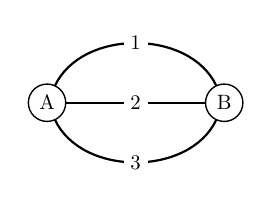
\begin{tikzpicture}[scale=0.75,transform shape]
  \Vertex[x=0,y=0]{A}
  \Vertex[x=3,y=0]{B}

  \tikzstyle{LabelStyle}=[fill=white,sloped]
  %Edges bend left
  \tikzstyle{EdgeStyle}=[bend left=65]		%\Edge[label=$120$](A)(B)  %if want to label the edge
      	\Edge[label=1](A)(B)
			
  %Edges bend right
  \tikzstyle{EdgeStyle}=[bend right=65]
	\Edge[label=3](A)(B)
  %Edges straight
  \tikzstyle{EdgeStyle}=[]
      \Edge[label=2](A)(B) 
\end{tikzpicture}

\caption{Graph $G$ of cities $A$ and $B$ connected by 3 routes.}
\label{2 cities}
\end{figure}

Thus we can see that the number of roundtrips $A \rightarrow B \rightarrow A$ using any of the edges $e \in \{1,2,3\}$ is given by 
$$\text{\# Roundtrips} = 3^n = 3^3 = 9$$

Alternatively, we could have computed it by counting all possible routes. Let $S$ be the set of all possible roundtrips from city $A$ to city $B$, where we can choose between routes 1, 2, and 3. Then the elements of $S$ are
$$S = \{11, 12, 13, 21, 22, 23, 31, 32, 33 \}$$

which has a cardinality $|S|$ of 9. If we are to restrict our roundtrip such that we must take a different route for the return trip, then we no longer can have the routes $\{11, 22, 33\}$. Therefore this subset $S'$ has a cardinality of
$$|S'| = |S| - 3 = 6$$


\section*{Question 2: Section 3.1 \#6}

For a linear (i.e. the first position and the $n$-th position are not adjacent) table of $n$ seats, we have $n$ ways to choose the first position, $n-1$ ways to choose the second position, .... , 1 way to choose the $n$-th position. This is equivalent to $n!$ ways to choose the arrangement of people. 

However, since this is a \textit{circular} table where there are no actual positions (only seating relative to each other), we have to fix the first person's position. Thus the remaining $n-1$ people can be arranged in $(n-1)!$ ways. This gives us a total of
$$1 \cdot (n-1)! = (n-1)!$$
ways to arrange $n$ people in a circular table.


\section*{Question 3: Section 3.1 \#7}

For a group of five people on an elevator that stops at five floors, let us assume that each has an equal probability of going to any one floor. Thus we can compute the probability that each person gets off at a different floor as
\begin{align*}
P(E) & = \frac{\text{\# ways assign distinct floors}}{\text{total \# ways assign floors}} \\
& = \frac{(n)_k}{n^k} \\
& = \frac{(5)_5}{5^5} \\
& = \frac{5 \cdot 4 \cdot 3 \cdot 2 \cdot (5-5+1)}{5 \cdot 5 \cdot 5 \cdot 5 \cdot 5} \\
& = \frac{24}{625} \\
& \approx 0.0384
\end{align*}


\section*{Question 4: Section 3.1 \#8}

\textbf{Proof:} For a finite set $\Omega$ of $n$ elements, the cardinality of the power set $\mathcal{P}(\Omega)$ is $2^n$.

Since the number of subsets is the summation of the unordered $k$-combinations for $k=0,1, \ldots , n$, we have that
$$|\mathcal{P}(\Omega)| = \sum_{k=0}^n {n \choose k}$$

From the Binomial Theorem, we know that
$$(x+y)^n = \sum_{k=0}^n {n \choose k} x^k y^{n-k}$$

Thus for $x=1$ and $y=1$, we can rewrite $2^n$ as
$$2^n = (1+1)^n = \sum_{k=0}^n {n \choose k} 1^k 1^{n-k} =  \sum_{k=0}^n {n \choose k}$$ \QEDA


\section*{Question 5: Section 3.1 \#12}

For a symphonic orchestra containing a repertoire of 30 Haydn symphonies, 15 modern works, and 9 Beethoven symphonies, a program must consist of a Haydn symphony followed by a modern work, and then a Beethoven symphony. Using this data, we can compute the following:

\begin{enumerate}[\qquad (a)]
	\item \textit{Total number of possible programs}
	
	Since there are 30 choices for the first position, 15 choices for the second position, and 9 choices for the third position, the number of programs is $30 \cdot 15 \cdot 9 = 4,050$.
	
	\item \textit{Number of programs if the pieces can be played in any order}
	
	For a 3-element set, the total number of permutations is $3! = 6$. Therefore if all 3 pieces can be played in any order, we have a total of
	$$4050 \cdot 6 = 24,300$$
	different programs.
	
	\item \textit{Number of programs if the pieces can be played in any order and more than one piece can be played from each category}
	
	If we remove the restrictions on the order and type of pieces played, then we simply have $n=30+15+9=54$ pieces that can be chosen for $k=3$ ways. Thus, the $3$-permutation is given by
	\begin{align*}
	(54)_3 & = \frac{54!}{(54-3)!} \\
	& =\frac{(54 \cdot 53 \cdot 52) \cdot 51!}{51!} \\
	& = 148,824
	\end{align*}	
\end{enumerate}


\section*{Question 6: Section 3.1 \#15}

For a computing centre, let there be 3 processors that receive $n$ jobs that are randomly assigned. The probability that exactly one processor has no jobs can be computed as
$$P(\text{1 processor no jobs}) = \frac{\text{\# ways assign processor no jobs}}{\text{total \# ways assign jobs}}$$

Since each of the 3 processors can be assigned $n$ jobs, we know that the total number of ways to assign jobs is $3^n$. For the number of ways to assign a processor no jobs, we can compute the number of ways to assign processor 1 no jobs and multiply this by the total number of processors:
\begin{align*}
	\text{\# ways assign processor no jobs} & = 3 \cdot (\text{\# ways assign processor 1 no jobs}) \\
	& = 3 \cdot (2^n) \\
\end{align*}
Thus we have
\begin{align*}
	P(\text{1 processor no jobs}) & = \frac{3 \cdot 2^n}{3^n} \\
	& = \frac{2^n}{3^{n-1}} \\
\end{align*}


\section*{Question 7: Section 3.1 \#17}

Among a set of $n$ people, we will assume that there are $k=12$ equiprobable choices for each person's birthday month. Let $E$ be the event that at least two people have their birthdays on the same month and $N$ be the event that no two people have their birthdays in the same month. Then the probability of event $E$ occurring may be expressed as
$$P(E) = 1 - P(N)$$

For $P(N)$, we have that
\begin{align*}
	P(N) & = \frac{\text{\# ways assign distinct birthdays}}{\text{total \# ways assign birthdays}} \\
	& = \frac{(12)_n}{12^n} \\
	& = \frac{12 \cdot 11 \cdot \ldots \cdot (12-n+1)}{12 \cdot 12 \cdot \ldots \cdot 12} \\
	& = 1 \cdot \Big(1 -\frac{11}{12}\Big) \cdot \ldots \cdot \Big(1- \frac{n-1}{12}\Big) \\
	& = \prod_{j=0}^{n-1} \Big(1- \frac{j}{12} \Big) \\
\end{align*}

Substituting this back into the equation for $P(E)$, we now have
$$P(E) = 1 - \prod_{j=0}^{n-1} \Big(1- \frac{j}{12} \Big)$$

\cleardoublepage

\section*{Question 8}

Let us denote the number of permutations in $S_n$ that have exactly $k$ fixed points by $w_n^{(k)}$, for all $k \geq 0$ and $n \geq 1$. First, we will compute the number of ways to arrange the $k$ fixed points. Since there are $n$ elements to be chosen for a $k$-element subset, we have $n \choose k$ permutations.

For the remaining $n-k$ points that must be arranged such that there are no fixed points, this is simply an $(n-k)$-derangement $w_{n-k}$.

Combining these, we have
$$w_n^{(k)} = {n \choose k} \cdot w_{n-k}$$

Using the above formula, we can calculate the probability that a random permutation in $S_n$ has exactly $k \geq 0$ fixed points to be
\begin{align*}
	P_n^{(k)} & = \frac{w_n^{(k)}}{n!} \\
	& = \frac{{n \choose k} \cdot w_{n-k}}{n!} \\
	& = \frac{\frac{n!}{k! \cdot (n-k)!} \cdot w_{n-k}}{n!} \\
	& = \frac{w_{n-k}}{k! \cdot (n-k)!} \\
\end{align*}
Since we know that
$$\lim_{n\to\infty} \frac{w_n}{n!} = \frac{1}{e}$$

Then we can compute the limit of $P_n^{(k)}$ as $n$ approaches infinity
\begin{align*}
	\lim_{n\to\infty} P_n^{(k)} & = \lim_{n\to\infty} \frac{w_{n-k}}{k! \cdot (n-k)!} \\
	& = \frac{1}{k!} \lim_{n\to\infty} \frac{w_{n-k}}{(n-k)!} \\
	& = \frac{1}{k!} \cdot  \frac{1}{e} \\
\end{align*}

and find that it approaches the constant $\frac{1}{e \cdot k!}$.



\end{document} 